\documentclass[a4paper,11pt]{ctexart}
\title{\Huge\textbf{《新概念物理题解》部分习题勘误}}
%\author{钟帅\ 编写 \\\\ 邓苏峰\ \  校对\\ 1.1 版本}
\author{1.2 版本}
\usepackage{graphicx}
\usepackage{fancyhdr}
\pagestyle{fancy}
%\lhead{
\includegraphics[scale=0.1]{logo.png}}
%在此处插入logo.pdf图片 图片靠左
\lhead{
\includegraphics[scale=0.2]{wy.jpg}} %if you prefer to use logo of weiyang
\chead{} % 页眉中间位置内容
\rightmark 
\usepackage{multirow}
\usepackage{amsmath}
\usepackage[colorlinks,linkcolor=red]{hyperref}
\usepackage{soul}
\usepackage{fontspec}
\usepackage[table,xcdraw]{xcolor}
\usepackage{amssymb,xtab}
\usepackage{url}
\usepackage[all,cmtip]{xy}
\usepackage{fontspec,xltxtra,xunicode,amsmath,amsthm,amssymb,mathrsfs,stmaryrd,eucal}


 \usepackage{color}

 \usepackage{yhmath}

\usepackage{graphicx}
\usepackage{amssymb}
\usepackage{bm}

\usepackage{ctex}
\graphicspath{{photo/}}

%定理环境
\usepackage{hyperref}
\usepackage{indentfirst}
\usepackage{url}


\newtheorem{thm}{定理}[section]
\newtheorem{lem}[thm]{引理}
\newtheorem{prop}[thm]{命题}
\newtheorem{propdefn}[thm]{命题-定义}
\newtheorem{cor}[thm]{推论}
\newtheorem{alg}[thm]{Algorithm}
\newtheorem{conj}[thm]{Conjecture}
\newtheorem{ques}[thm]{习题}
\newtheorem{prop-defn}[thm]{Proposition-Definition}
\newtheorem{clm}[thm]{Claim}
%\theoremstyle{definition}
\newtheorem{defn}[thm]{定义}
\newtheorem{const}[thm]{Construction}
\newtheorem{exam}[thm]{例}
\newtheorem{rem}[thm]{注}
\newtheorem{warn}[thm]{Warning}
%\theoremstyle{remark}
\newtheorem{thesis}[thm]{Thesis}


\newtheorem{notation}[thm]{记号}


\renewcommand{\proofname}{证明:}


\begin{document}
\maketitle

\begin{figure}[b]
    \centering
\begin{minipage}[t]{0.48\textwidth}
    \centering
    
\includegraphics[scale=1.55]{wy.jpg}    
\end{minipage}
\begin{minipage}[t]{0.48\textwidth}
    \centering
    
\includegraphics[scale=0.31]{无标题.jpg}    
\end{minipage}

\end{figure}

%\newpage


\newpage
\tableofcontents

\newpage

\part{说明}
\paragraph{}
本勘误针对2009年6月第1版的《新概念物理题解》(上册)(下册)力学与光学部分。
勘误范围仅包括ChenShaomin老师2022年春季学期基础物理学(1)的教学日历中布置的作业。
\paragraph{}
勘误的主要内容由未央水木-12班的钟帅编写,同班的邓苏峰同学进行了校对。
编写此勘误的最初想法是作为本班女生节的惊喜,当然如果能帮助到更多同学就更好了。
\paragraph{}
《新概念物理》系列教材的质量其实还是相当高的,本勘误内指出的大部分的错误只是一些打印或者题意理解上的问题,
不代表书中一定不对(有可能是编者自己的理解不够全面),未进行勘误的内容也不能代表书中一定正确(有可能是编者也做错了或者勘误范围中没有涉及)。
由于编写时间比较短,内容上可能还存在一定的问题,如果读者有补充勘误或者发现了勘误中的错误,欢迎将补充内容通过\href{https://cloud.tsinghua.edu.cn/u/d/201c674f93ed4445929c/}{未央-水木12学习资料上传链接}上传。感谢!

\paragraph*{2022年12月24日补充说明}
为支援\href{https://weyoung-learn.github.io/}{未央学习}项目,编者将该项目上传至github,
并计划寒假补上ChenShaomin老师基物(2)的内容。
后续发现的问题欢迎通过\href{https://github.com/OscarZs/Corrigendum-to-Basic-Physics}{基物勘误}项目反馈。


\part{力学}
\section{力学第一章\ 质点运动学}
\paragraph{暂未发现错误}

\section{力学第二章\ 动量守恒\ 质点动力学}
\paragraph{暂未发现错误}

\section{力学第三章\ 机械能守恒}
\paragraph{习题3-25}类型:方法补充\\
原题目中的公式$v_n = v_o(1-e^{-\frac{2n\delta m}{m}})$可能乍一看上去不是那么显然
,实际上它适用于$\delta m \to \infty $(也就是把粒子流视为连续体)的极限情况。\\
下面给出从这个角度进行推导的思路:\\
由题意中的$\delta m \ll m$,可以联想到将每次碰撞视为一个微元过程。
每次碰撞前后,
\begin{equation*}
    \frac{v+dv}{v_0} = \frac{2 dm}{m+dm}+\frac{m-dm}{m + dm} \frac{v}{v_0}
    \footnote{上式用到了弹性碰撞的公式,可以由动量守恒与能量守恒推导出来,此处不再展开}
\end{equation*}
展开并忽略m的二阶小量,得到
\begin{equation*}
    \frac{dv}{v-v_o } = -\frac{2dm}{m_0}
\end{equation*}
积分
\begin{equation*}
    \int_{0}^{v}\frac{dv}{v-v_o} = -\int_{0}^{n\delta m}\frac{2dm}{m_0}
\end{equation*}
即可得到
\begin{equation}
    v_n = v_o(1-e^{-\frac{2n\delta m}{m}})
\end{equation}
这样处理可能会更直观。$\alpha n \to \infty$时,也能得到$v_n \to v_0$.\\
题解说$\alpha n \to \infty$时公式(1)不适用。
这里讨论的其实是当$\alpha n \to \infty$时,\\
$(1-\alpha)^n$与$ e^{-\alpha n }$之间是否近似相等。
\\由于$\alpha \ll 1$,
\begin{equation*}
    e^{-\alpha} = (1- \alpha)+o(\alpha)
\end{equation*}
当n不够大时,(1)式即等价于题目所给的
\begin{equation}
    v=v_0(1-b^n)
\end{equation}而后者实际上对任何粒子质量$\delta m$都适用,
不需要$\delta m \ll m$的限制。
\\$n \to \infty$时,(1)(2)的差异被放大,此时使用(1)就不合适了。

\section{力学第四章\ 角动量守恒}
\paragraph{习题4-4}类型:题意不清晰\\
题解的思路可以判断当$l$变化时$v$、$\sin{\theta}$的变化,
但按照题意,应该是要用$l_1$、$l_2$、$v_1$来表示$v_2$ 的。
由于按照原题意处理在数学上比较复杂,建议直接按照题解的意思来完成此题。

\paragraph{习题4-7}类型:答案错误\\
题解开头就写错了,应为
\begin{equation*}
    l_{1c}=\frac{m_2l}{m_1+m_2},l_{2c}=\frac{m_1l}{m_1+m_2}
\end{equation*}
最终答案应为
\begin{equation*}
    \frac{J_{1C}}{J_{2C}} =\frac{m_2}{m_1}<1
\end{equation*}

\paragraph{习题4-25}类型:计算错误
$T_2$的表达式有误,应为

\begin{equation*}
    T_2=\frac{I+m_1R(R+r)}{I+m_1R^2+m_2r^2}
\end{equation*}


\paragraph{习题4-36}类型:题意理解\\
题解对“用力”的理解采用的是给平板一个加速度,编写者认为“抽”的过程其实更类似于给一个冲量。
当然无论采用那种理解,主要都是要找到滑动、滚动等状态的临界点进行分析。

\section{力学第五章\ 连续体力学}
\paragraph{习题5-11}类型:计算错误\\
原题解积分错误,应该改为\\
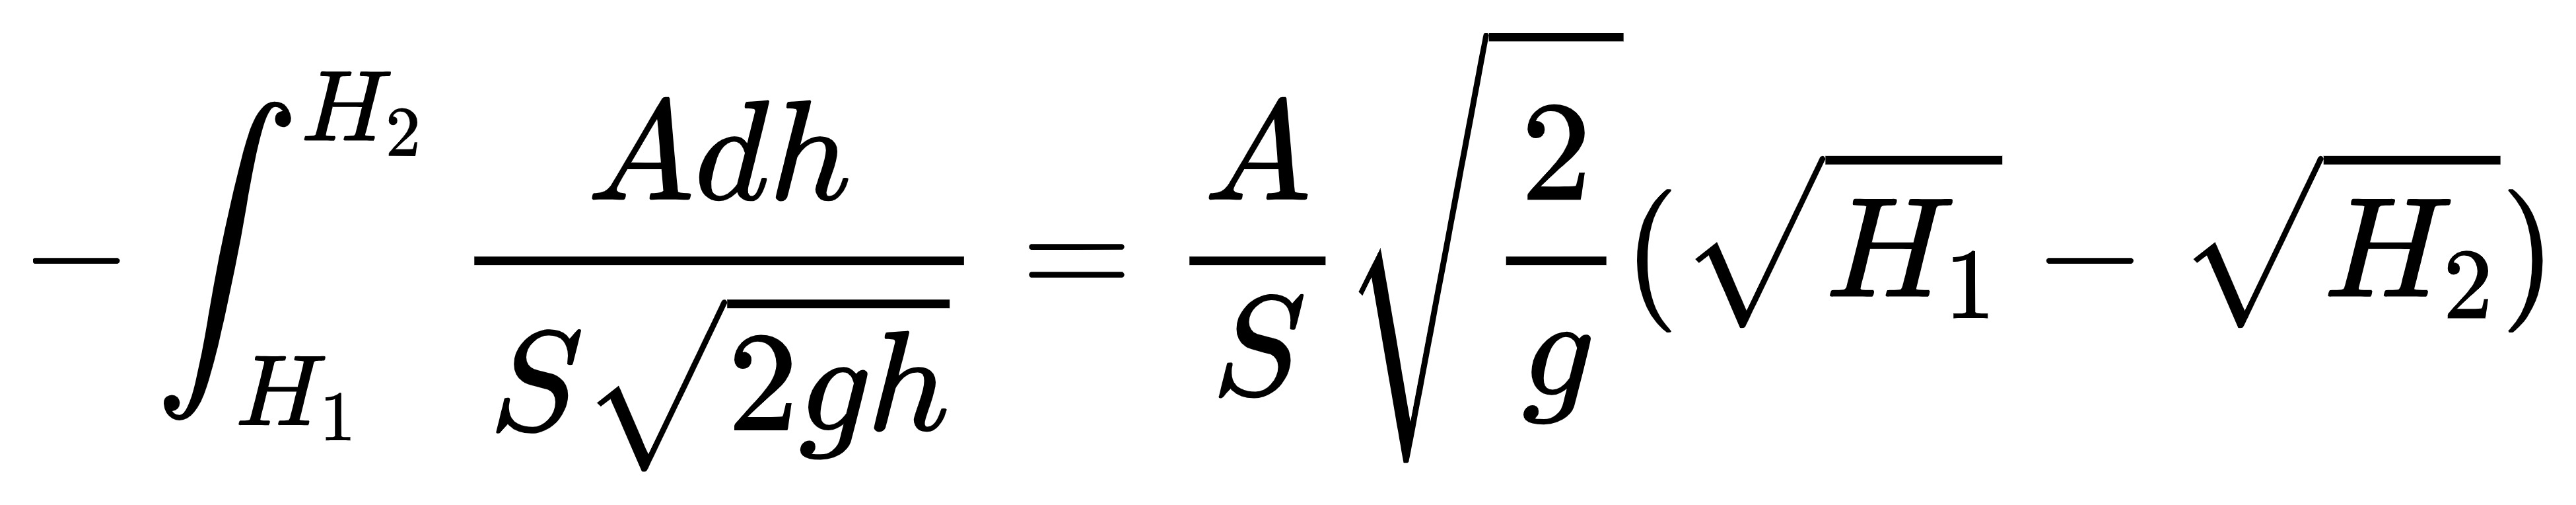
\includegraphics[scale = 0.045]{1.jpg}
\footnote{这张图有点奇怪是因为overleaf突然解决不了根号里面有分式的公式了,所以编者直接插入了图片。}\\
所以最后答案都是原来的4倍。

\paragraph{习题5-12}类型:计算错误\\
套用了上一问的公式,上一问算错了这一问也就跟着错了。\\
答案是原答案的4倍。

\section{力学第六章\ 振动和波}
\paragraph{习题6-4}类型:计算错误\\
(2)问中$\sin{(-\frac{\pi}{2})} = -1 \neq 0$,正确答案应为$F(0)=3.75 \times 10^{-4}N$

\paragraph{相位问题}类型:概念理解\\
本章几道要求相位的题目都没有给表达式,默认为余弦的相位。\\
编者未找到相关的规定,建议自己回答时先写清楚表达式再写对应的相位。

\section{力学第七章\ 万有引力}
\paragraph{习题7-5、习题7-6、习题7-8}类型:计算精度\\
这一部分的习题在计算过程中保留的位数较少,对最后答案的影响较大。\\(但其实也不能说是错误)\\
依照编者的计算,\\
习题7-5的答案应为$1.28 \times 10^{3} kg/m^{3}$.\\
习题7-6的答案应为3.30h.\\
习题7-8的答案应为27.35min.\\

\section{力学第八章\ 相对论}
\paragraph{习题8-9、8-20、8-23}类型:常量取值与计算精度\\
本章不少题目将光速$c_0$取为$3 \times 10^8$,可能会导致有的题目答案最后两位上出现差异,可以多留意。当然也有的题是因为与前一章相同的计算精度的问题而产生了偏差。\\
依照编者计算,\\
习题8-9的答案为$0.976c_0$。\\
习题8-20的答案为20.71u.\\
习题8-23的答案为24.75d。\\

\paragraph{习题8-11}类型:常量取值\&计算错误\\
$A_1$处取值错误,$A_1=0.005m_0c^2=4.13\times10^{-16}$ J\\
$A_2$处计算错误,$A_2=0.627m_0c^2=5.14\times10^{-14}$ J


\part{光学}
\section{光学第一章\ 光和光的传播}
\paragraph{暂未发现错误}

\section{光学第二章\ 几何光学成像}
\paragraph{习题2-6}类型:符号规则\\
此题中$r < 0$,应对应凹面镜。\\\\
其实对于正物距,凸面镜是不可能成实像的。据此也就很容易发现题解的问题。\\
初学几何光学也需要多注意符号规则,尝试自己推导出一套符号规则。
自己推导的符号规则记忆更深、更便于检验,会比死记正负、虚实、凹凸之间的关系更有效。
(当然啦,首先你推导的公式要自洽)

\section{光学第三章\ 干涉}
\paragraph{习题3-5}类型:一些细节上的小问题\\
本题(2)(3)问用$\frac{\Delta l}{\Delta x} $来计算条纹数目。有的题目会将0级条纹设定在中点处,因而条纹数目会是$\frac{\Delta l}{\Delta x} \pm 1$。
当然后者的考虑也过于理想了,实验中也不太可能达到。编者认为纠结这类问题其实没什么意义,写出来也仅供参考。\\\\
再者就是这道题(2)(3)的题目默认忽略了双镜尺寸带来的影响。题干中加一句“认为双镜尺寸足够大”显得更严谨一些

\paragraph{习题3-19}类型:计算错误\\
这道题其实应该是题目和题解的部分内容打错了,题解是按照$\lambda=550.0nm$来处理的。\\
按照题目给的$500.0nm$,计算结果应该为\\
$h =(2k-1)96.2nm \\$
$\delta_1 = 1.25(2k-1) \pi $\\
$\delta_2 = 0.71(2k-1) \pi $\\

\paragraph{习题3-22}类型:计算错误\\
最后一步的计算有错误,应为\\
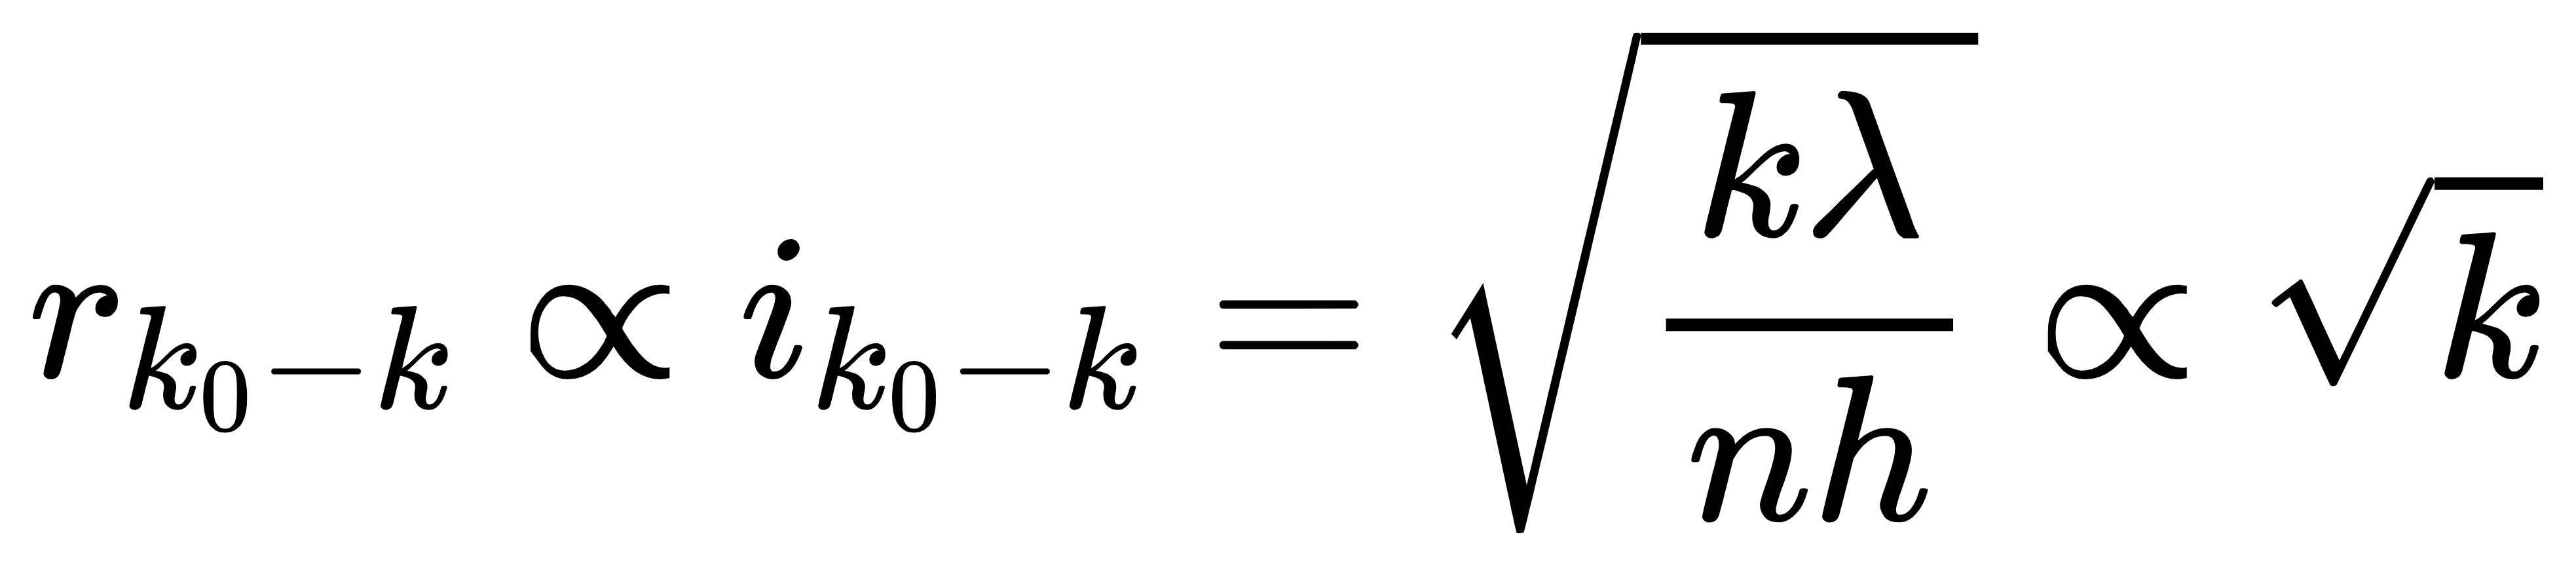
\includegraphics[scale = 0.04]{2.jpg}


%\section{problem 1}
%\begin{thm}[勾股定理]
%    如果$a$,$b$,$c$为直角三角形的三边长,那么有:
%   \[a^2+b^2=c^2
%    \]
%\end{thm}
%\begin{proof}
%    如图,这几乎是显然的。
%    \begin{figure}[h]
%        \centering
%        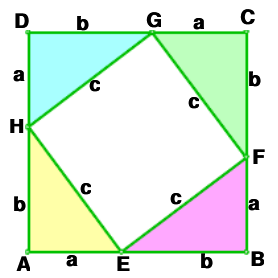
\includegraphics{gougu.png}
%    \end{figure}
%\end{proof}


\end{document}